\documentclass[fontsize=12pt, % Document font size
               paper=a4, % Document paper type
               hyperref]{report}

%\usepackage[bottom=10em]{geometry} % Reduces the whitespace at the bottom of the page so more text can fit
\usepackage[margin=1.0in]{geometry} % Reduces the whitespace at the bottom of the page so more text can fit

\usepackage[english]{babel} % English language
\usepackage{lipsum} % Used for inserting dummy 'Lorem ipsum' text into the template

\usepackage[utf8]{inputenc} % Uses the utf8 input encoding
\usepackage[T1]{fontenc} % Use 8-bit encoding that has 256 glyphs

%\usepackage[osf]{mathpazo} % Palatino as the main font
%\linespread{1.05}\selectfont % Palatino needs some extra spacing, here 5% extra
%\usepackage[scaled=.88]{beramono} % Bera-Monospace
%\usepackage[scaled=.86]{berasans} % Bera Sans-Serif
%\usepackage[euler-digits]{eulervm}

\usepackage{booktabs,array} % Packages for tables

\usepackage{amsmath, amsfonts} % For typesetting math
\usepackage{graphicx} % Required for including images
\usepackage{etoolbox}
\usepackage[norule]{footmisc} % Removes the horizontal rule from footnotes
\usepackage{lastpage} % Counts the number of pages of the document
\usepackage{xifthen}

%\usepackage{natbib}

\usepackage[dvipsnames]{xcolor}  % Allows the definition of hex colors
\definecolor{titleblue}{rgb}{0.16,0.24,0.64} % Custom color for the title on the title page
%\definecolor{linkcolor}{rgb}{0,0,0.42} % Custom color for links - dark blue at the moment
\definecolor{linkcolor}{RGB}{155,0,0}
\definecolor{citecolor}{RGB}{0,100,115}
\definecolor{urlcolor}{RGB}{89,22, 175}
%\definecolor{linkcolor}{red!50!black}
%\definecolor{citecolor}{blue!50!black}
%\definecolor{urlcolor}{blue!80!black}

\DeclareFixedFont{\textcap}{T1}{phv}{bx}{n}{1.5cm} % Font for main title: Helvetica 1.5 cm
\DeclareFixedFont{\textaut}{T1}{phv}{bx}{n}{0.8cm} % Font for author name: Helvetica 0.8 cm

\usepackage[nouppercase,headsepline]{scrpage2} % Provides headers and footers configuration
\pagestyle{scrheadings} % Print the headers and footers on all pages
\clearscrheadfoot % Clean old definitions if they exist

\automark[chapter]{chapter}
\ohead{\headmark} % Prints outer header

\setlength{\headheight}{25pt} % Makes the header take up a bit of extra space for aesthetics
\setheadsepline{.4pt} % Creates a thin rule under the header

\ofoot[\normalfont\normalcolor{\thepage\ |\  \pageref{LastPage}}]{\normalfont\normalcolor{\thepage\ |\  \pageref{LastPage}}} % Creates an outer footer of: "current page | total pages"

% For color boxes
\usepackage{tcolorbox}

% For chemistry
\usepackage{mhchem}

% Hyperlink configuration
\usepackage[
    pdfauthor={}, % Your name for the author field in the PDF
    pdftitle={Laboratory Journal}, % PDF title
    pdfsubject={}, % PDF subject
    bookmarksopen=true,
    linktocpage=true,
    urlcolor=linkcolor, % Color of URLs
    citecolor=linkcolor, % Color of citations
    linkcolor=linkcolor, % Color of links to other pages/figures
    backref=page,
    pdfpagelabels=true,
    plainpages=false,
    colorlinks=true, % Turn off all coloring by changing this to false
    bookmarks=true,
    pdfview=FitB]{hyperref}

\usepackage[stretch=10]{microtype} % Slightly tweak font spacing for aesthetics

%\setlength\parindent{0pt} % Uncomment to remove all indentation from paragraphs

%----------------------------------------------------------------------------------------
%       NEW COMMANDS
%----------------------------------------------------------------------------------------
% Convenience Macros
\newcommand{\KL}{Karhunen-Lo\`{e}ve}

% Comments
\newcommand{\dls}[1]{\textcolor{red}{DLS: #1}} % Comments from David

\newcommand{\commentout}[1]{}

% General math operators
\newcommand{\lr}[1]{\left(#1\right)}  % Left-right parentheses
\newcommand{\pdeone}[2]{\frac{\partial #1}{\partial #2}} % First partial derivative
\newcommand{\pden}[3]{\frac{\partial^{#3} #1}{\partial #2^{#3}}} % n-th order partial derivative (user specifies n)
\newcommand{\odeone}[2]{\frac{\mathrm{d} #1}{\mathrm{d} #2}} % First order ordinary derivative
\newcommand{\oden}[3]{\frac{\mathrm{d}^{#3} #1}{\mathrm{d} #2^{#3}}}  % n-th order ordinary derivative (user specifies n)
\renewcommand{\div}{\nabla\cdot} % Divergence operator
\newcommand{\dx}[1]{\ \mathrm{d}#1} % Differential in integral
\renewcommand{\time}{\mathrm{t}} % Time variable
\newcommand{\tr}{\mathrm{tr}} % Transpose operation
\newcommand{\mean}[1]{\overline{#1}} % Mean of a quantity
\newcommand{\ave}[1]{\left<#1\right>} % Average operator
\newcommand{\Nl}{N_{\ell}} % Number of Legendre modes
\newcommand{\ev}[1][]{%
  \ifthenelse{\equal{#1}{}}{\lambda}{\lambda_{#1}}
} % Eigenvalues
\newcommand{\efk}[1]{\varphi_{#1}} % Eigenmodes (index notation)
\newcommand{\ef}[1]{\boldsymbol{\varphi}_{#1}} % Eigenmodes (vector)

% Fluids operators
\newcommand{\vel}{\mathbf{u}} % Velocity vector
\newcommand{\stress}{\boldsymbol{\tau}} % Stress tensor in momentum equation
\newcommand{\diffvel}{\mathbf{V}} % Diffusion velocity
\newcommand{\Yk}[1]{Y_{#1}} % Species mass fraction
\newcommand{\grav}{\mathbf{g}} % Force of gravity
\newcommand{\fa}[1]{\widetilde{#1}} % Favre average
\newcommand{\ff}[1]{#1^{\prime\prime}} % Favre fluctuations
\newcommand{\ra}[1]{\bar{#1}} % Reynolds average
\newcommand{\diss}{\epsilon} % Dissipation
\newcommand{\Ceo}{C_{\diss 1}} % First dissipation coefficient
\newcommand{\Cet}{C_{\diss 2}} % Second dissipation coefficient
\newcommand{\Stk}{S_{kT}} % Turbulent Schmidt number of species k
\newcommand{\Y}{\mathbf{Y}} % Vector of species mass fractions
\newcommand{\chist}{\chi_{\mathrm{st}}} % Stoichometric scalar dissipation

% Kinetics operators
\newcommand{\Wk}{W_{k}} % Molecular weight
\newcommand{\rrk}[1]{\dot{\omega}_{#1}} % Species reaction rates
\newcommand{\rrT}{\dot{\omega}^{\prime}_{T}} % Reaction rate term in energy equation
\newcommand{\nur}{\nu_{kj}^{\prime}} % Reverse stoichiometric coeff
\newcommand{\nup}{\nu_{kj}^{\prime\prime}} % Forward stoichiometric coeff
\newcommand{\nukj}[1]{\nu_{kj}} % Difference in stoichiometric coeffs
\newcommand{\xk}[2]{%
\ifthenelse{\isempty{#2}{}}{x_{#1}}{x_{#1}^{#2}}%
}
\newcommand{\xc}[1][]{%
  \ifthenelse{\equal{#1}{}}{\mathbf{x}}{\mathbf{x}^{#1}}%
}
\newcommand{\enth}[1][]{%
\ifthenelse{\equal{#1}{}}{\mathbf{h}}{\mathbf{h}^{#1}}%
}
\newcommand{\ent}[1][]{%
\ifthenelse{\equal{#1}{}}{\mathbf{s}}{\mathbf{h}^{#1}}%
}
\newcommand{\cp}[1][]{%
\ifthenelse{\equal{#1}{}}{\mathbf{c}_{p}}{\mathbf{c}_{p}^{#1}}%
}
\newcommand{\rr}[1][]{%
  \ifthenelse{\equal{#1}{}}{\dot{\boldsymbol{\omega}}}{\dot{\boldsymbol{\omega}}^{#1}}
}% Reaction rate vector
\newcommand{\rri}[1][]{%
  \ifthenelse{\equal{#1}{}}{\dot{\boldsymbol{\upsilon}}}{\dot{\boldsymbol{\upsilon}}^{#1}}
}% Inadequacy vector

\newcommand{\kf}{k_{j}^{\lr{f}}} % Forward reaction rate
\newcommand{\kr}{k_{j}^{\lr{r}}} % Reverse reaction rate
\newcommand{\ke}{k_{j}^{\lr{e}}} % Reverse reaction rate
\newcommand{\pr}[1]{q_{#1}} % Progress rate of reaction
\newcommand{\cpk}[1]{c_{p#1}} % Specific heat (constant p)
\newcommand{\hk}[1]{h_{#1}} % Enthalpy of species
\newcommand{\sk}[1]{s_{#1}} % Entropy of species
\newcommand{\heating}{\dot{\mathcal{Q}}} % Heating rate in energy equation
\newcommand{\Sop}{\boldsymbol{\mathcal{S}}} % Linear stochastic operator
\newcommand{\Aop}{\boldsymbol{\mathcal{A}}} % Virtual reactions

% Combustion operators
\newcommand{\flame}{\mathbf{U}} % Flamelet solution vector

\newcommand{\flamek}[1][]{%
  \ifthenelse{\equal{#1}{}}{U}{U_{#1}}
} % Flamelet solution

% Statistic operators
\newcommand{\rz}{\omega} % Realization
\newcommand{\prob}[1]{p\lr{#1}} % General probability distribution
\newcommand{\covar}[1]{\mathcal{C}_{#1}} % Covariance
\newcommand{\param}{\boldsymbol{\theta}} % Generic parameter vector
\newcommand{\normal}[2]{\mathcal{N}\lr{#1, #2}} % normal distribution
\newcommand{\lnormal}[2]{\mathrm{ln}\mathcal{N}\lr{#1, #2}} % lognormal distribution

















\begin{document}

\title{\textcolor{titleblue}{Chemical Kinetics Mistakes} \\[1cm]}

\author{David Sondak}
\date{} % No date by default, add \today if you wish to include the publication date

\maketitle % Title page

\newpage % Start lab look on a new page

\pagestyle{scrheadings} % Begin using headers

\section{Initial Formulation}
  The initial formulation of our inadequacy model for chemical 
  kinetics was a generalization of the original stochastic operator 
  inadequacy model~\cite{morrison2016representing}.  We began by
  introducing a simple global temperature dependence into the 
  stochastic inadequacy operator.

  The following subsections describe the intial chemical 
  kinetics formulation~\ref{sec:chemkin1}, review the original 
  inadequacy operator~\ref{sec:inad1}, and discuss the introduction 
  of the global temperature depenence~\ref{sec:inad1}.  Following 
  this review, we discuss the drawbacks of this approach and 
  motivate an alternative formulation~\ref{sec:discuss1}.
  

  \subsection{Chemical Kinetics} \label{sec:chemkin1}
  We consider a mixture at temperature $T$ undergoing $M$ elementary 
  reactions and consisting of $N$ species.  The chemical system is
  given by~\cite{kee2005chemically}
  \begin{align}
    \sum_{k=1}^{N}{\nur\mathcal{M}_{k}} \ce{<=>} 
    \sum_{k=1}^{N}{\nup\mathcal{M}_{k}}, 
    \quad j = 1,\ldots,M \label{eq:reactions}
  \end{align}
  where $\nur$ and $\nup$ represent the molar stoichiometric 
  coefficients of the reactants and products, respectively and 
  $\mathcal{M}_{k}$ is the symbol for species $k$.  The species molar 
  concentrations are $\xc\lr{\time}$.  The $k^{\mathrm{th}}$ 
  component of $\xc$ is the molar concentration of the species 
  corresponding to $\mathcal{M}_{k}$.  
  
  Given the set of reactions~\eqref{eq:reactions}, the evolution of the
  molar concentrations in a perfectly stirred reactor is governed by the
  following set of ODEs:
  \begin{align}
     \odeone{\xc}{\time} = \rr\lr{\xc, T} \label{eq:ode_reactions}
  \end{align}
  where $\rr\lr{\xc, T}$ is the vector of reaction rates.  The reaction 
  rate of species $k$ is
  \begin{align}
    \rrk{k} = \sum_{j=1}^{M}{\nukj{kj}\pr{j}}, \qquad k = 1,\ldots,N,
    \label{eq:rrk}
  \end{align}
  where $\pr{j}$ is the progress rate of reaction $j$ and $\nukj{kj} =
  \nup - \nur$ is the difference between product and reactant
  stoichiometric coefficients.  The progress rate $\pr{j}$ depends on
  the forward and reverse reaction rates, $\kf$ and $\kr$ respectively
  as well as the molar concentration of each species and has the form
  \begin{align}
    \pr{j} = \kf\prod_{k=1}^{N}{\displaystyle\xk{k}{\nur}} - 
             \kr\prod_{k=1}^{N}{\displaystyle\xk{k}{\nup}}, 
    \qquad j = 1,\ldots,M.
  \end{align}
  The forward reaction rate is given by a modified Arrhenius 
  reaction as
  \begin{align}
    \kf = A_{j}T^{b_{j}}\exp\lr{-E_{j}/RT}, 
    \qquad j = 1,\ldots,M, 
    \label{eq:arrhenius}
  \end{align}
  where $R$ is the ideal gas constant.  The Arrhenius parameters $A_{j}$, $b_{j}$ and $E_{j}$ 
  are the Arrhenius prefactor, modified Arrhenius parameter, and activation energy and are the 
  uncertain reaction rate parameters.  The reverse reaction rate can be written in terms of the 
  forward rate,
  \begin{align}
    \kr = \frac{\kf}{\ke}, \qquad j = 1,\ldots,M
  \end{align}
  where $\ke$ is the equilibrium constant.  The equilibrium 
  constant is determined via thermodynamic considerations.  We 
  refer the reader to~\cite[Ch.9.3]{kee2005chemically} for specific 
  details on its development.  The final form for $\ke$ is 
  \begin{align}
    \ke = \lr{\frac{p_{a}}{RT}}^{\sum_{k=1}^{N}{\nukj{kj}}}
          \exp\lr{\frac{\Delta \sk{j}}{R} - \frac{\Delta \hk{j}}{RT}}, 
    \qquad j = 1,\ldots,M \label{eq:ke}
  \end{align}
  where $p_{a}$ is atmospheric pressure, $\Delta \sk{j}$ is the 
  change in entropy for reaction $j$ and $\Delta \hk{j}$ is the 
  change in enthalpy for reaction $j$.  The entropy and enthalpy 
  for each species are determined from the specific heat for each 
  species $\cpk{k}\lr{T}$,
  \begin{subequations}
    \begin{align}
      \hk{k}\lr{T} &= \int{\cpk{k}\dx{T}}, \qquad k = 1,\ldots,N \\
      \sk{k}\lr{T} &= \int{\frac{\cpk{k}}{T}\dx{T}}, \qquad k=1,\ldots,N
    \end{align}
  \end{subequations}
  and the specific heat is represented by a polynomial curve fit of 
  order $p$, 
  \begin{align}
    \cpk{k}\lr{T} = \sum_{i=0}^{p}{\alpha_{ki}T^{i}}, \qquad k = 1,\ldots,N.
  \end{align}
  A common polynomial form in combustion is the NASA
  polynomials~\cite{mcbride1993coefficients} where $p=7$ or $p=9$.  The coefficients 
  $\alpha_{ki}$ are determined from experimental measurements or theory when available.  
  Once the enthalpies and entropies of each species are available the change in entropy 
  and enthalpy for a given reaction is 
  \begin{subequations}
    \begin{align}
      \Delta \hk{j} = \sum_{k=1}^{N}{\nukj{kj}\hk{k}\lr{T}}, \qquad j = 1,\ldots,M \\
      \Delta \sk{j} = \sum_{k=1}^{N}{\nukj{kj}\sk{k}\lr{T}} \qquad j=1,\ldots,M.
    \end{align}
  \end{subequations} 
  At this point, only temperature has been left unspecified.  The temperature of 
  the mixture is determined from the energy equation,
  \begin{align}
    \odeone{T}{\time} = \dfrac{-\displaystyle\enth\lr{T}\cdot\rr\lr{\xc,T} + \heating}
                              {\displaystyle\cp\lr{T}\cdot\xc} 
    \label{eq:energy}
  \end{align}
  where $\heating$ is a user-prescribed heating rate.

    
  \subsection{Inadequacy Formulation} \label{sec:inad1}
  Combustion chemistry is well known to be highly complex, often
  involving tens of species and hundreds of reactions for even seemingly
  simple fuels~\cite{kee2005chemically}.  In some cases, the true
  chemistry is sufficiently complicated that high-fidelity chemical
  models are unknown.  Further, even when a sufficiently high-fidelity,
  detailed chemical model is available, it may involve so many species
  and reactions as to be computationally intractable for use in practical 
  combustion simulations.  In such a case, it is common to replace the 
  detailed mechanism with a reduced model containing fewer species and 
  reactions.  In either case, when performing practical combustion simulations, 
  it is common for the chemical kinetics representation to introduce
  non-negligible modeling error.
  
  In the approach being pursued here, these errors are quantified
  probabilistically using the stochastic model inadequacy 
  operator~\cite{morrison2016representing}.  This approach is intended to
  address the two major sources of modeling error in chemical models:
  missing chemical species and missing reaction pathways.  To represent
  the possible effects of the missing species, the original chemical
  model state is enriched with virtual species---one for each type of
  atom in the system.  To represent the possible effects of missing
  pathways, a stochastic perturbation of the original chemical model
  reaction mechanism involving both the original species and the virtual
  species is formulated.  The goal of this work is to extend these ideas
  from preveious work~\cite{morrison2016representing} to practical combustion
  simulations.
  
  To illustrate the ideas in a concrete but simple setting, we consider
  \ce{H2}/\ce{O2} combustion.  The twenty-one reaction, eight species
  model~\cite{williams2008detailed} is taken to be a
  high-fidelity model, and the five reaction, seven species model
  from~\cite{williams2008detailed} is used as the chemical model for
  which we wish to develop an inadequacy representation.  This setting
  enables straightforward assessment of the model inadequacy
  representation.

  In light of these sources of uncertainty, we are developing a physics-based inadequacy 
  model for chemical kinetics.  The goal of the inadequacy formulation is twofold.  First, 
  it should account for the effects of the missing reaction pathways and species while not 
  representing them directly.  Secondly, it should provide a way forward for prediction 
  of quantities of interest such as $\ce{NO_x}$ generation.  Our approach follows the 
  philosophy for validating prediction of unobserved quantities of interest as described 
  in~\cite{oliver2015validating}.  We begin the development of the inadequacy model by 
  introducing a hierarchy of models for chemical kinetics that follow the evolution 
  equations~\eqref{eq:ode_reactions} and~\eqref{eq:energy}, 
  \begin{align}
    &\odeone{\xc[H]}{\time} = \rr[H]\lr{\xc[H],T} \\
    &\odeone{T}{\time} = \dfrac{-\displaystyle\enth[H]\lr{T}\cdot\rr[H]\lr{\xc[h],T} + \heating}
                              {\displaystyle\cp[H]\lr{T}\cdot\xc[H]}.
  \end{align}
  The superscript index $H$ can take values of $D$, $R$ and $I$ referring, respectively, to 
  the detailed model, the reduced model and the inadequacy model.  In this work, the detailed 
  model is taken to be a surrogate for the truth and has $N_{D}$ species with $M_{D}$ reactions.
  Similarly, the reduced model has $N_{R}$ species and $M_{R}$ reactions while the inadequacy 
  model has $N_{I}$ species and $M_{I}$ reactions.  The species in the reduced model are 
  $\left\{\ce{H2}, \ce{O2}, \ce{H}, \ce{O}, \ce{OH}, \ce{HO2}, \ce{H2O}\right\}$ and the 
  reduced reaction set is 
  \begin{align*}
    \ce{H + O2 <=> O + OH} \\
    \ce{O + H2 <=> H + OH} \\
    \ce{H2 + OH <=> H2O + H} \\
    \ce{H + O2 + M <=> HO2 + M} \\
    \ce{H2 + O2 <=> HO2 + H}
  \end{align*}
  where $\ce{M}$ is a third body.
  
  
  The inadequacy model developed herein is a probabilistic model and is
  formulated as an enrichment of the reduced model.  The fact that it is
  probabilistic means that it depends on realizations of stochastic
  parameters which we denote abstractly as $\rz$.  We will comment
  further on the stochastic nature of the inadequacy model when we
  introduce its specific form.  First, we introduce $N_{a}$ virtual
  species where $N_{a}$ is equal to the number of atoms in the system.
  Hence, the total number of species in the system is $N_{I} = N_{R} +
  N_{a}$.  The \ce{H2}-\ce{O2} system has two atoms (\ce{H} and \ce{O})
  and so $N_{a} = 2$.  Let $\xc[v] : \mathbb{R} \to \mathbb{R}^{N_{a}}$
  and let $\ce{H^{\prime}}$ and $\ce{O^{\prime}}$ denote the virtual
  species.  The virtual species are proxies for \ce{H} and \ce{O}.
  Their purpose is to provide a mechanism to capture the effects of
  neglected species.  With the introduction of the virtual species we
  now let $\rr[I] : \mathbb{R}^{N_{I}}\times\mathbb{R} \to
  \mathbb{R}^{N_{I}}$.  Moreover, we augment $\rr[R]$ with the zero
  vector of size $N_{a}$.  The augmented vector is $\rr[R]_{0} =
  \left[\rr[R], \ \mathbf{0}\right]^{tr}$.  Let $\rri :
  \mathbb{R}^{N_{I}}\times\mathbb{R} \to \mathbb{R}^{N_{I}}$ denote the
  perturbation of the reduced model right hand side.  The species
  evolution equation is now
  \begin{align}
    \odeone{\xc[I]}{\time} = \rr[I]\lr{\xc[I], T} \label{eq:ode_inad}
  \end{align}
  where 
  \begin{align}
    \rr[I]\lr{\xc[I], T} = \rr[R]_{0}\lr{\xc[R], T} + \rri\lr{\xc[I], T; \rz}. \label{eq:rr_inad}
  \end{align}
  
  Recent work~\cite{morrison2016representing} introduced a stochastic operator for $\rri$.  The 
  idea was to introduce a linear correction to the reduced model as well as three additional 
  reaction pathways that facilitate movement of the virtual species.  The stochastic operator 
  takes the form
  \begin{align}
    \rri\lr{\xc[I]} = \Sop\xc[I] + \Aop\lr{\xc[I]} \label{eq:inad_model_noT}
  \end{align}
  where $\Sop$ is a stochastic linear operator that represented
  additional reaction pathways not included in the reduced model.
  Requirements for $\Sop$ to conserve atoms and preserve positivity of
  species concentrations are discussed in detail by Morrison et
  al.~\cite{morrison2016representing}.  
  
  Note that $\Sop$ permits species in the model to react to form other
  species or virtual species.  By involving the virtual species, one has
  the potential to represent the effects of real species not included the
  model and associated pathways.  However, the linearity of $\Sop$ has
  the undesirable side-effect that, in some cases, mass can become such
  in the virtual species.  To avoid this problem, the nonlinear operator
  $\Aop$ is added.  In the \ce{H2}-\ce{O2} system $\Aop$
  represents the following reactions,
  \begin{align}
    \ce{H^{\prime} + O^{\prime}  ->[\kappa_{1}] OH} \\
    \ce{H^{\prime} + 2O^{\prime} ->[\kappa_{2}] HO2} \\
    \ce{H^{\prime} + O^{\prime}  ->[\kappa_{3}] H2O}
  \end{align} 
  where $\kappa_{j}$ is the constant forward reaction rate for the reaction.  Note that 
  these reactions do not proceed in the reverse direction.
  
  While this new model form represents an enrichment of the original
  model, there is no expectation that the new form is correct in a
  deterministic sense.  That is, we do not expect that there are
  universal values of the entries of $\Sop$ and rate parameters
  $\kappa_j$ that perfectly correct the model.  Instead, the required
  values will vary from case to case.  To develop a model that is
  applicable to a wide range of scenarios, we represent this variability
  by modeling the entries of $\Sop$ and $\kappa_i$ as random variables
  with given probability distributions parameterized by additional
  hyperparameters.  These hyperparameters are inferred based on data
  using a hierarchical Bayesian approach.
  
  The present inadequacy
  operator~\eqref{eq:inad_model_noT} does not contain any temperature
  dependence.  In this way, the operator is always active even for
  temperatures when no reactions are occurring and when the reduced model
  is performing well.  This feature leads to qualitatively incorrect
  results for some problems.  For instance, in a laminar counterflow
  diffusion flame case, the inadequacy operator is active even well
  outside the flame, where there should be no uncertainty.  In an
  attempt to overcome this limitation we introduce a global temperature
  dependence $g\lr{T}$ on the inadequacy operator,
  \begin{align}
    \rri\lr{\xc[I]} = g\lr{T}\left[\Sop\xc[I] + \Aop\lr{\xc[I]}\right]. \label{eq:inad_model_T}
  \end{align}
  It is also possible to introduce temperature dependence into each of the entries of $\Sop$ 
  but this would increase the dimensionality of the system considerably which we wish to 
  avoid.  Moreover, the global temperature dependence offers a clean way to introduce the 
  desired temperature control on the inadequacy model.  We introduce two forms for $g\lr{T}$.  
  The first form is a global Arrhenius temperature dependence, 
  \begin{align}
    g_{A}\lr{T} = \exp\lr{-\frac{T_{\mathrm{ag}}}{T}} \label{eq:gA}
  \end{align}
  where $T_{\mathrm{ag}}$ is a global activation temperature and is inferred as part of the 
  calibration procedure.  The second form for $g\lr{T}$ that we consider is a global 
  switch, 
  \begin{align}
    g_{S}\lr{T} = \tanh\lr{T - T_{\mathrm{on}}} - \tanh\lr{T - T_{\mathrm{off}}} \label{eq:gS}
  \end{align}
  where $T_{\mathrm{on}}$ and $T_{\mathrm{off}}$ are two additional parameters to be calibrated.

  We briefly comment on our calibration approach for the kinetics inadequacy model.  We use a 
  hierarchical Bayesian method in which, for certain parameters, we propose a specific 
  probability distribution characterized by parameters (called hyperparameters) and we calibrate the 
  hyperparameters in addition to the parameters themselves.  Our approach is inspired by 
  techniques pioneered in the statistics community~\cite{berliner1996hierarchical} but our 
  interpretation is slightly different.  To illustrate the procedure and our interpretation, 
  we provide an example.
  
  Bayes' theorem is 
  \begin{align}
    \prob{\left.\param\right| \mathbf{D}} = 
    \frac{\prob{\left.\mathbf{d} = \mathbf{D}\right|\param}\prob{\param}}{\prob{\mathbf{D}}}
    \label{eq:bayes}
  \end{align}
  where $\prob{\left.\mathbf{d} = \mathbf{D}\right|\param}$ is the likelihood function, 
  $\prob{\param}$ is the prior probability density function for the parameters and 
  $\prob{\left.\param\right| \mathbf{D}}$ is the posterior probability distribution of 
  the parameters.  $\prob{\mathbf{D}}$ is called the evidence and is treated as a 
  normalization factor in most algorithms.  A particular value of the truth data $\mathbf{D}$ 
  is denoted by $\mathbf{d}$ and $\param$ denotes a vector of parameters.  We provide 
  prior distributions that represent our prior knowledge of the system.  For example, 
  for purely positive parameters one may propose a log-normal distribution.  In order to 
  illustrate the hierarchical approach that we use, we will work with a normal distribution.  
  Note that parameters in the stochastic operator do not strictly use normal distributions.  
  For the specific prior distributions, the reader is referred to~\cite{morrison2016representing}.  
  
  A normally-distributed parameter $\theta$ with mean $\mu$ and standard deviation $\sigma$ 
  has the prior distribution,
  \begin{align}
    \prob{\theta} \sim \normal{\mu}{\sigma^{2}}. \label{eq:normal_prior}
  \end{align}
  In the hierarchical approach, the mean and variance $\eta = \sigma^{2}$ are also 
  distributions.  In the present work, the mean is also normally distributed while 
  the variance is given by the uninformative Jeffreys distribution, 
  \begin{subequations}
    \begin{align}
      \mu        &\sim \normal{\mu_{\mu}}{\sigma^{2}_{\sigma}} \\
      \sigma^{2} &\sim \mathcal{J}.
    \end{align}
  \end{subequations}
  The hierarchical approach is beneficial because we do not wish the calibration of the 
  inadequacy model to apply to a single problem.  By calibrating the hyperparameters, 
  the inadequacy model can be used in various scenarios that may differ from the 
  calibration scenario.  Note that we directly calibrate the parameters appearing 
  in the global temperature dependence.
  
  In the present work, we choose a Gaussian likelihood function, 
  \begin{align}
    \prob{\left.\mathbf{d} = \mathbf{D}\right|\param} = 
    \exp\lr{-\frac{1}{2}\lr{\mathbf{y} - \mathbf{d}}^{\tr}\boldsymbol{\Sigma}\lr{\mathbf{y} - \mathbf{d}}} 
    \label{eq:lhood}
  \end{align}
  where $\mathbf{y}$ is the prediction from the kinetics model and $\mathbf{d}$ is 
  truth data from the detailed model.  The matrix $\boldsymbol{\Sigma}$ contains 
  observation errors for each field (concentration and temperature).  
  
  The results only include a calibration of 
  the inadequacy model.  Calibration of the Arrhenius reactions was not performed in 
  this analysis since we were only interested in the effects of the calibrated 
  inadequacy model.  The standard deviation of the prior distributions was taken to be 
  $10\%$ of the mean values.  The inverse problem~\eqref{eq:bayes} was solved using the 
  delayed rejection adaptive Metropolis (DRAM) algorithm provided in the QUESO software 
  package~\cite{mcdougall2015parallel, estacio2016queso}.

  The posterior distributions were propagated through the model~\eqref{eq:ode_inad} and 
  the accompanying energy equation.  Figure~\ref{fig:T_evo} shows the time-evolution of 
  the temperature of the mixture from the maximum likelihood estimate of each calibrated 
  inadequacy model.  The solution from the detailed model is compared to that from the 
  reduced model and various versions of the inadequacy model.  The inadequacy model without 
  any temperature dependence ($g\lr{T} = 1$) is shown in the left plot of Figure~\ref{fig:T_evo}.  
  We observe that when using~\eqref{eq:inad_model_noT} as the inadequacy model the mixture 
  ignites almost immediately.  This is precisely the issue we wish to address by introducing a 
  temperature dependent inadequacy model.  We also observe that the final temperature is far too 
  high when compared with the detailed model.  On the other hand, in the right plot of 
  Figure~\ref{fig:T_evo}, which is zoomed to the ignition time, we observe that the global 
  Arrhenius temperature dependence delays ignition but that the ignition time is delayed almost 
  to that of the reduced model which does not match the detailed model.  Finally, the global 
  switch temperature dependence performs somewhat better relative to the detailed model but still 
  does not correctly predict the ignition time.
  \begin{figure}[h!]
    \begin{center}
      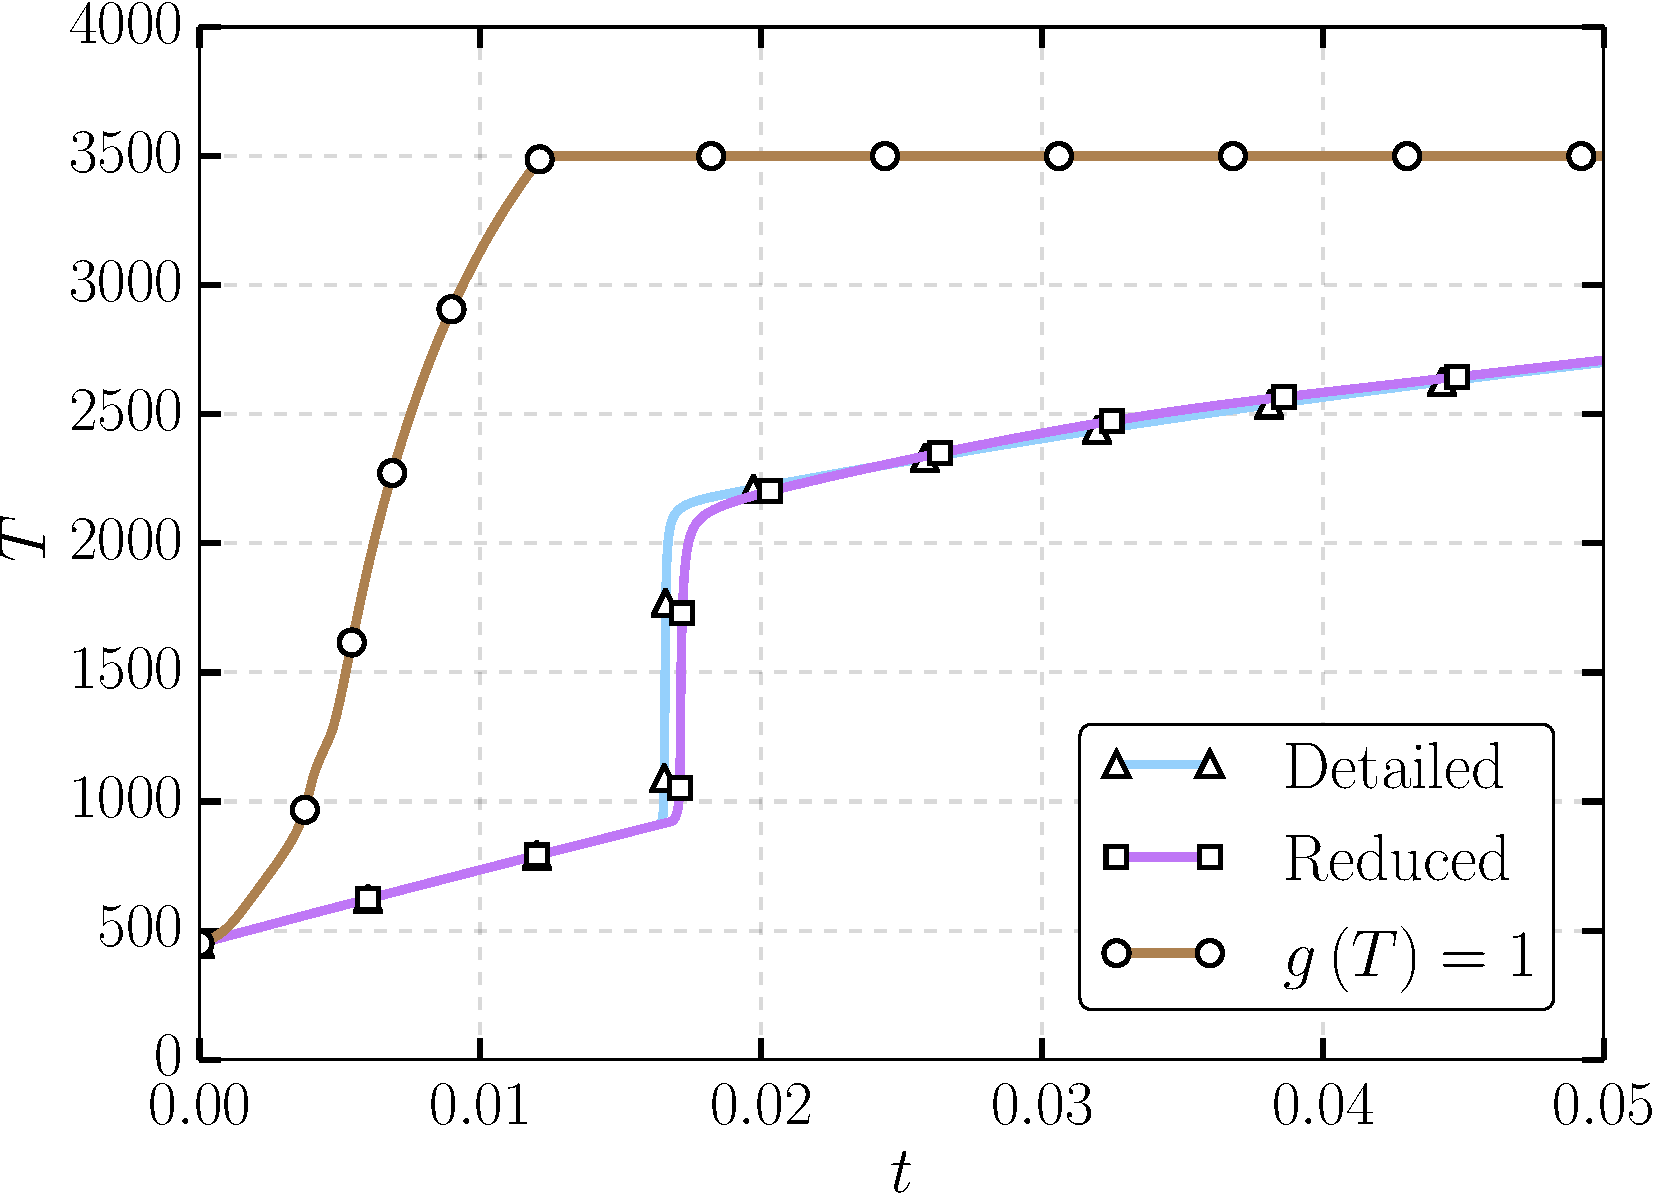
\includegraphics[width=0.49\linewidth]{T_evo_unity.pdf}~
      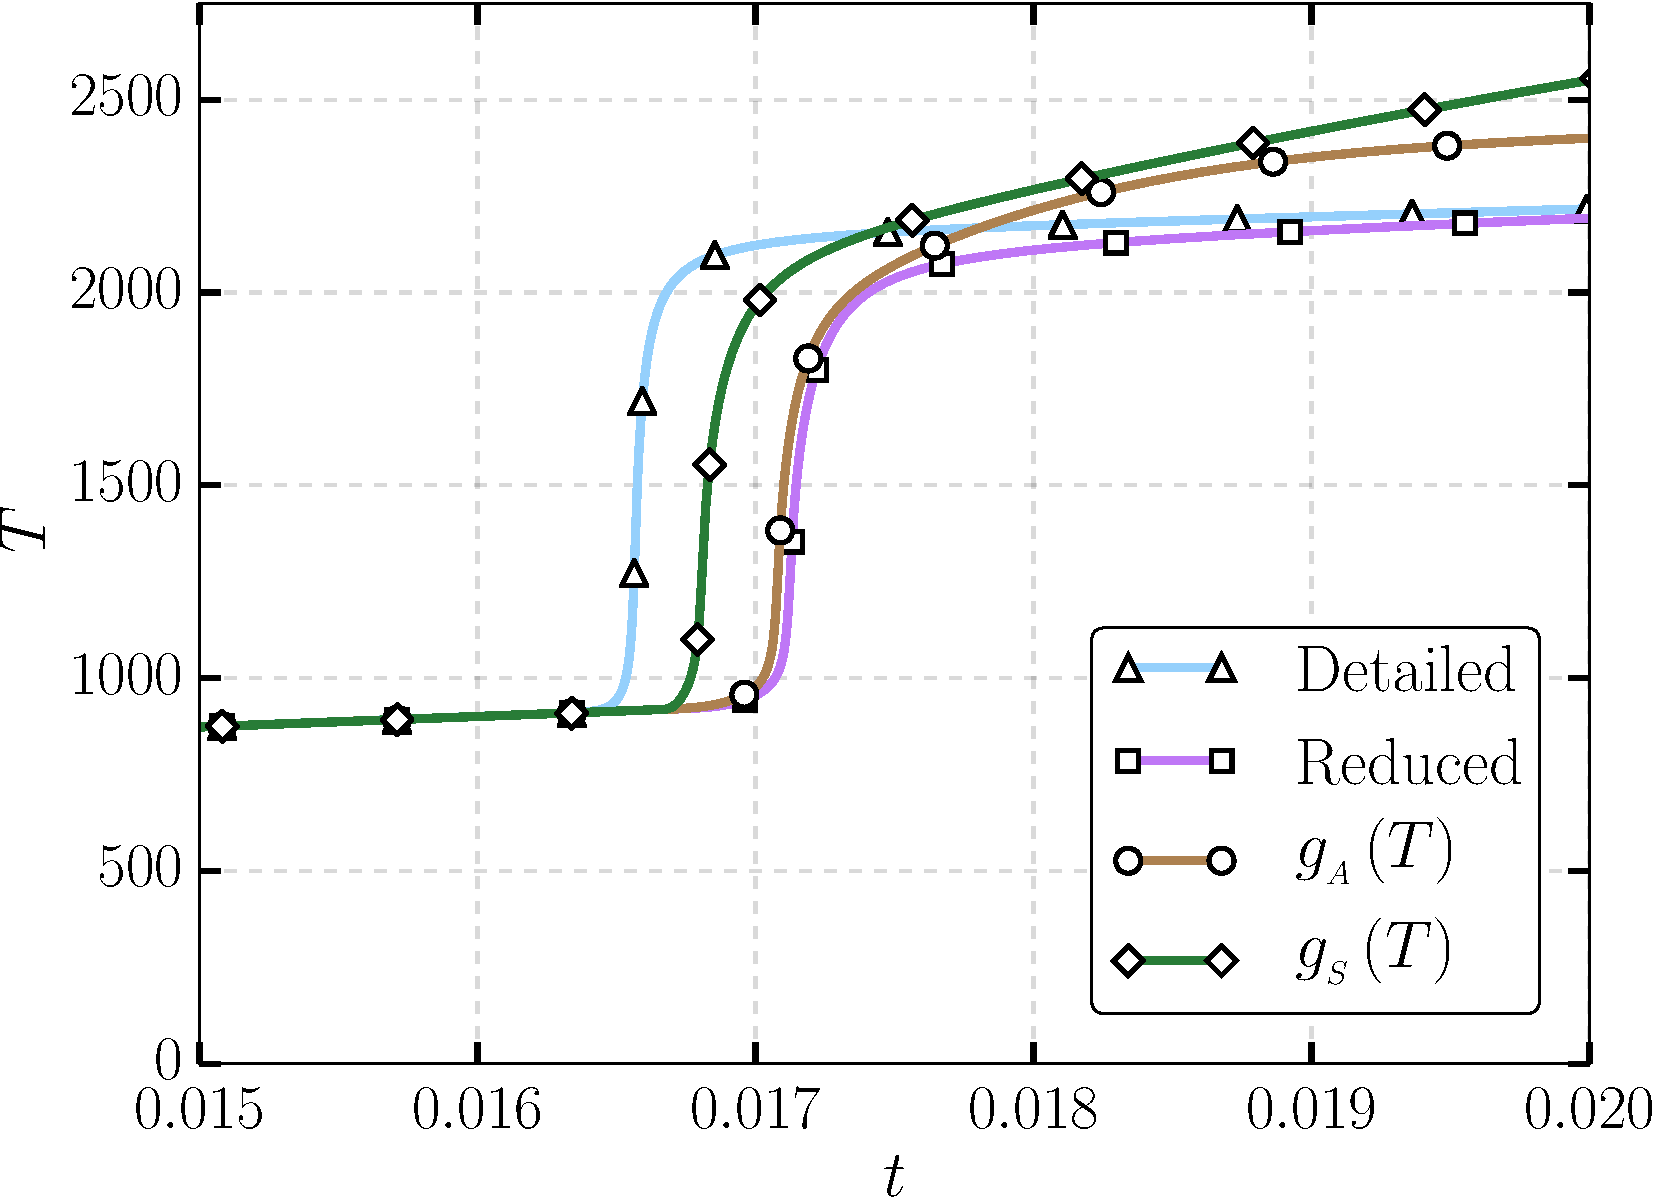
\includegraphics[width=0.49\linewidth]{T_evo_global.pdf}
    \end{center}
    \caption{Time evolution of the temperature in the perfectly stirred reactor. 
             The detailed model and reduced model are provided for reference.  
             A deterministic forward solve using parameters from the maximum 
             likelihood estimate of the inadequacy model without (left) and 
             with (right) global temperature dependence.}
    \label{fig:T_evo}
  \end{figure}
  
  Based on the results from a deterministic forward solve using parameters from the 
  maximum likelihood estimate, we decided to assess the performance of the global switch 
  temperature dependence.  Figure~\ref{fig:tanh_inadequacy} plots the time evolution of the 
  temperature.  Each solution is zoomed to the ignition time as before.  The 
  detailed model solution and the reduced model solution are provided as reference.  
  The mean of the solutions obtained using the calibrated global switch model 
  captures the ignition time very well although it misses the equilibrium behavior.  
  We also considered credibility interval curves at the $40\%$ and $90\%$ confidence 
  intervals.  Figure~\ref{fig:tanh_inadequacy} shows that there is an enormous spread in the 
  data between these curves.  The spread is so large that model only indicates that 
  the mixture may or may not ignite.  We therefore note that the temperature-dependent 
  inadequacy model~\eqref{eq:inad_model_T}, although flexible, does not provide predictive 
  capabilities.
  \begin{figure}[h!]
    \centering
    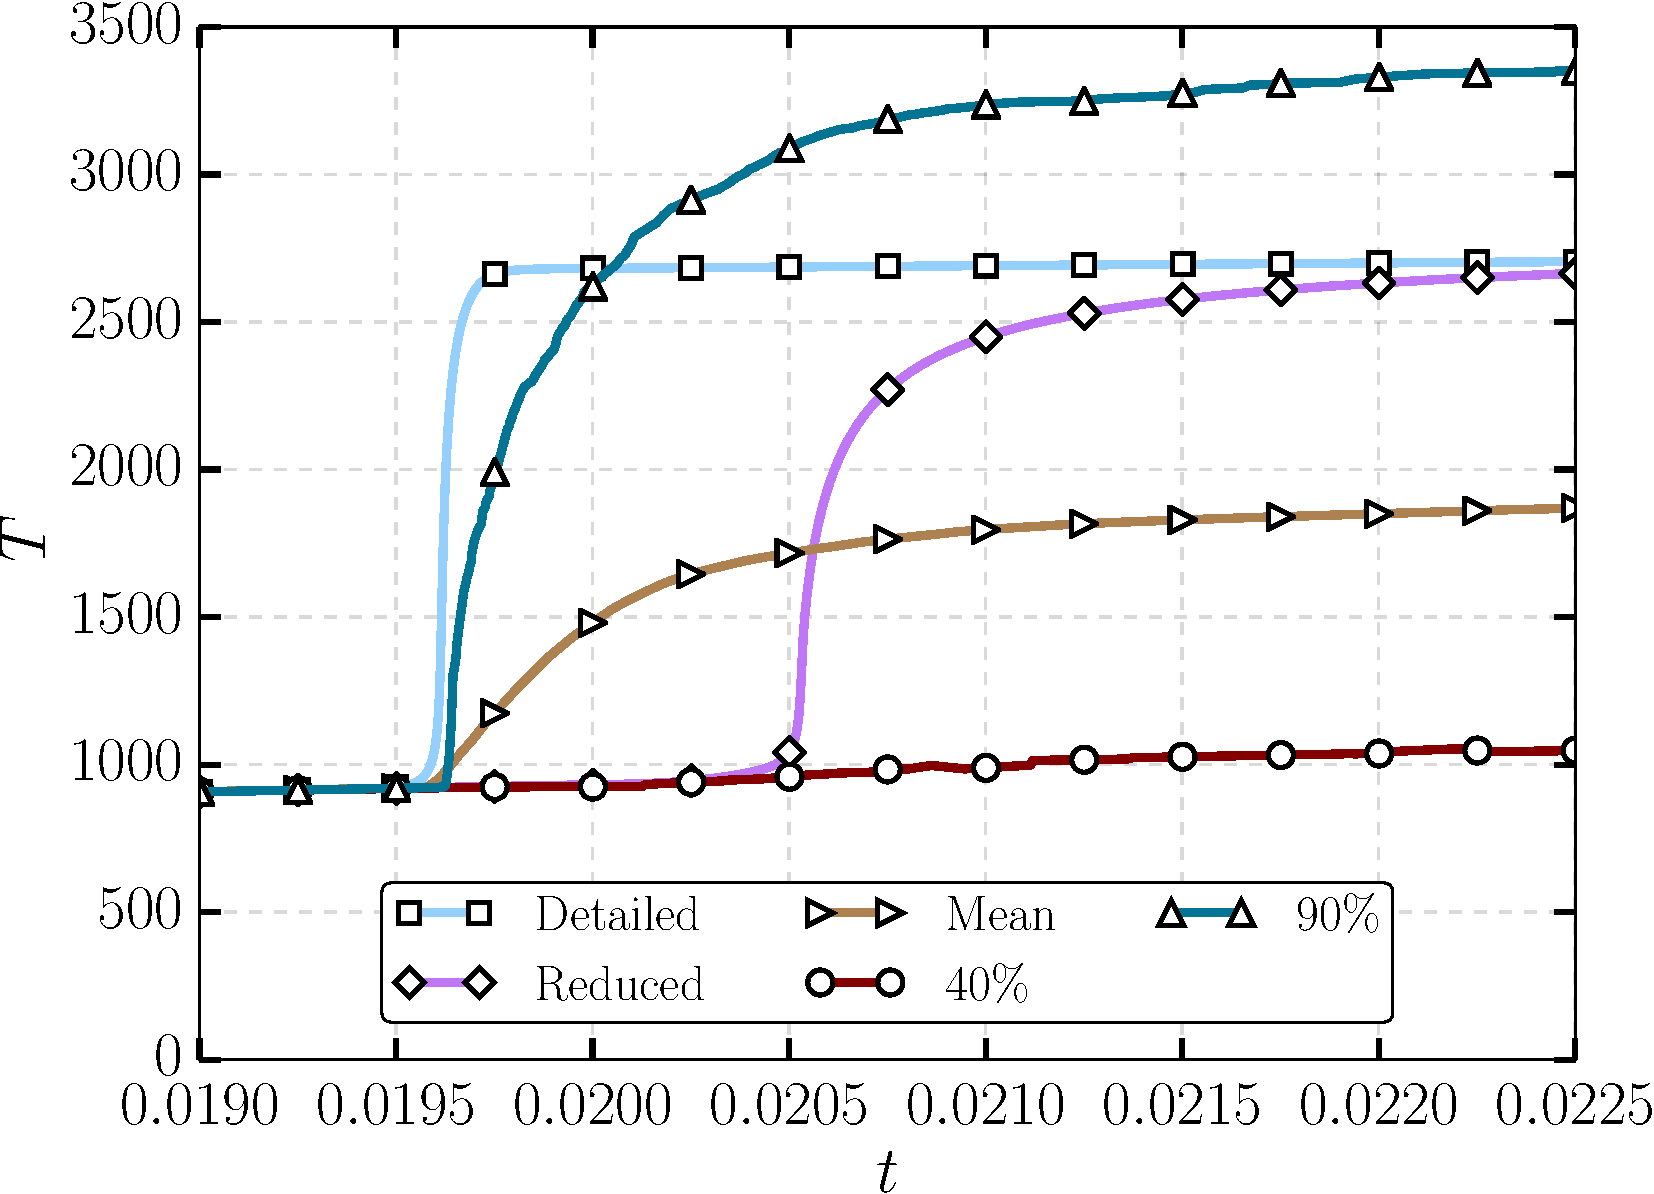
\includegraphics[width=0.6\textwidth]{tanh_inadequacy.pdf}
    \caption{Time evolution of temperature in the perfectly stirred reactor. 
             The mean of the results from the calibrated global switch model 
             captures the ignition time very well.  However, the overall 
             model fails to provide meaningful prediction capabilities.}
    \label{fig:tanh_inadequacy}
  \end{figure}


  \subsection{Discussion} \label{sec:discuss1}
  The lack of predictive capabilities of the temperature-dependent
  inadequacy operator indicates that a new inadequacy model is likely
  required.  In particular, at least with the data used for this
  calibration, the resulting model predictions are so uncertain as to be
  not useful.  Further, given that the original reduced model predicts
  the chemical equilibrium result quite well, the large uncertainty
  predicted at later times shown in Figure~\ref{fig:tanh_inadequacy} is
  unnecessary.  Thus, it appears that a richer dependence of the
  stochastic model on the thermochemical state is required.  Such a
  formulation should allow different inadequacy reactions to be active
  at different times and may need to be fully nonlinear.

\section{First Reformulation}
  One possible route to including richer temperature dependence in the 
  inadequacy model involves expanding the role of the virtual species.  
  Doing so provides a way of introducing a fully nonlinear inadequacy model 
  which provides additional reaction pathways that mimic the effects of the 
  those pathways that have been neglected from the detailed model.  We have 
  begun work on an inadequacy model that consists of a set of reversible 
  dissociation-recombination reactions.  Each species in the reduced model 
  is able to dissociate into the virtual species.  The virtual species can 
  then recombine to form the actual species.  In such a formulation, 
  formation of the virtual species should not be preferred since they are 
  only used as a placeholder for missing reaction pathways.  As such, the 
  recombination reactions should be favored.  To accomplish this, the 
  thermochemical parameters for the virtual species must be carefully 
  constrained.  One manner of constraint is require the Gibbs free energy 
  for each reaction in the virtual reaction set to be positive.  This 
  constraint in turn places additional constraints on the thermochemical 
  parameters of the virtual species.

  Recall that the original stochastic operator formulation introduced a set 
  of virtual species whose original purpose was to provide an outlet for 
  atoms that would belong to neglected species.  Put another way, the virtual 
  species attempt to account for the missing mass that may be 
  neglected in the reduced model.  For example, in the \ce{H2}/\ce{O2} 
  system used in the present work, \ce{H2O2} is neglected in 
  the reduced model.  However, atoms belonging to \ce{H2O2} may 
  dissociate into other species which \textit{are} present in the 
  reduced model.  An additional and important benefit of introducing 
  the virtual species is that they provide possible additional reaction 
  pathways. 


  \subsection{Chemical Kinetics} \label{sec:chemkin2}
  The initial chemical kinetics formulation presented in Section~\ref{sec:chemkin1} 
  did not apply to the combustion application we have in mind.  
  The formulation that we are interested in consists of a constant 
  pressure reactor whose volume may change in time.  The gas mixture 
  in the chamber is assumed to follow the ideal gas law 
  \begin{align}
    pV = X R T \label{eq:ideal_gas_law}
  \end{align}
  where $p$ is the constant reactor pressure, $V = V\lr{t}$ is 
  the volume of the reactor, $X$ represents the total moles in 
  the mixture, $R$ is the ideal gas constant and $T$ is the 
  temperature of the mixture.  We consider a mixture of $N$ 
  species undergoing $M$ reactions.  Note that the total 
  moles in the mixture is simply the sum of the moles of each 
  species, 
  \begin{align}
    X = \sum_{k=1}^{N}{\moles{k}}.
  \end{align}
  
  The total moles of each species evolves according to 
  \begin{align}
    \odeone{\moles{k}}{\time} = \rrk{k}V
  \end{align}
  where the reaction rate is still governed by~\eqref{eq:rrk}.
  The energy equation is now 
  \begin{align}
    \odeone{T}{\time} = \frac{-\enth\cdot\rr V + \heating}{\cp\cdot\x}
  \end{align}
  where $\enth$ is the enthalpy of each species in molar units, 
  $\cp$ is the specific heat at constant pressure for each 
  species (also in molar units), $\heating$ 
  is the user-supplied heating rate (a constant in what follows), 
  and $\x$ is the number of moles of each species. 

  

  \subsection{Inadequacy Formulation}
  The most obvious choice for 
  the virtual species is one for each atom in the system.  For the 
  \ce{H2}/\ce{O2} system the set of virtual species is 
  $\xv = \left(\ce{H}^{\prime}, \ce{O}^{\prime}\right)$.  We posit that 
  this minimal set of species will provide enough flexibly to meet 
  our goals.  There are a variety of possibilities for incorporating 
  the virtual species into a reaction set.  We focus on a set of 
  $M_{v}$ dissociation-recombination reactions.  We allow each species in 
  the system to dissociate into its constituent atoms which are represented 
  by the virtual species.  Moreover, we propose that the virtual species 
  can recombine into their parent species.  The species in the reduced model 
  for the \ce{H2}/\ce{O2} system are 
  $\left\{\ce{H2}, \ce{O2}, \ce{H}, \ce{O}, \ce{OH}, \ce{HO2}, \ce{H2O}\right\}$. 
  There are five non-monatomic species in the reduced model leading to 
  $M_{v}=5$ virtual reactions.  The set of reversible, dissociation-recombination 
  virtual reactions is therefore
  \begin{align}
    \ce{H2}  &\ce{<=>} 2\Hp \tag{VR1} \label{eq:VR1} \\
    \ce{O2}  &\ce{<=>} 2\Op \tag{VR2} \label{eq:VR2} \\
    \ce{OH}  &\ce{<=>} \Hp + \Op \tag{VR3} \label{eq:VR3} \\
    \ce{HO2} &\ce{<=>} \Hp + 2\Op \tag{VR4} \label{eq:VR4} \\
    \ce{H2O} &\ce{<=>} 2\Hp + \Op \tag{VR5} \label{eq:VR5}.
  \end{align}
  
  The set of virtual reactions is treated as a set of reversible 
  modified Arrhenius reactions.  That is, the forward reaction 
  rates for reactions~\eqref{eq:VR1}-\eqref{eq:VR5} are 
  \begin{align}
    \kf{j} = A_{j}T^{b_{j}}\exp\lr{-E_{j}/RT}, \qquad j = 1,\ldots M_{v}
  \end{align}
  where the set of kinetics parameters $\left\{A_{j}, b_{j}, E_{j}\right\}$ 
  have proposed distributions with hyperparameters that are to be 
  inferred.  We must also provide a way of representing the 
  enthalpy and specific heat of each virtual species in order to 
  determine the mixture temperature.  The 
  specific heat for each virtual species is prescribed in the form
  \begin{align}
    c_{pk}^{\prime} = \alpha_{k1} + 2\alpha_{k2}T, \qquad k = 1,\ldots,N_{v}.
  \end{align} 
  The enthalpy and entropy for each species are then 
  \begin{align}
    h_{k}^{\prime} &= \alpha_{k0} + \alpha_{k1}T + \alpha_{k2}T^{2}, 
      \qquad k = 1,\ldots,N_{v} \\
    s_{k}^{\prime} &= \beta_{k} + \alpha_{k1}\ln\lr{T} + 2\alpha_{k2}T, 
      \qquad k = 1,\ldots,N_{v}.
  \end{align}
  The coefficients $\alpha_{ki}$ and $\beta_{k}$ will also be
  given proposed distributions with associated hyperparameters 
  to infer.  Before outlining the inference procedure, we 
  introduce additional information about the virtual 
  reactions~\eqref{eq:VR1}-\eqref{eq:VR5}.  In particular, 
  we wish to ensure that the reverse reaction is favored 
  over the forward reaction so that recombination of 
  virtual species into actual species is favored.  This constraint 
  can be enforced by considering the Gibbs free energy for reaction 
  $j$, 
  \begin{align}
    \Delta G_{j}^{\lr{v}}= \Delta h_{j} - T \Delta s_{j}, 
      \qquad j = 1, \ldots, M_{v}.
  \end{align}
  Note that $\Delta G_{j}^{\lr{v}}$ can be expressed in terms of the 
  Gibbs free energy of each species as 
  \begin{align}
    \Delta G_{j}^{\lr{v}} &= \sum_{k=1}^{N}{\nu_{kj}\lr{h_{k} - T s_{k}}} \\
                 &= \sum_{k=1}^{N}{\nu_{kj}g_{k}}
  \end{align}
  where $h_{k}$ and $s_{k}$ are the enthalpy and entropy of 
  each species in the system including the virtual species.
  The reverse reaction is favored if $\Delta G_{j}^{\lr{v}} > 0$.  
  We use this constraint on our virtual reactions to constrain 
  the entropy constants $\beta_{k}$.  Any parameters 
  appearing in the thermochemistry representation for the actual 
  species are taken to be immutable.  The constraints on the 
  entropy coefficients are 
  \begin{align}
    \beta_{_{\ce{H}^{\prime}}} &< \underbrace{-s_{_{\ce{H}^{\prime}}}^{\lr{T}} + 
          \frac{1}{T}\left[h_{_{\ce{H}^{\prime}}} - \frac{1}{2}g_{_{\ce{H2}}}\right]}_{\displaystyle c_{1}}
      \label{eq:c1} \\
    \beta_{_{\ce{O}^{\prime}}} &< \underbrace{-s_{_{\ce{O}^{\prime}}}^{\lr{T}} + 
          \frac{1}{T}\left[h_{_{\ce{O}^{\prime}}} - \frac{1}{2}g_{_{\ce{O2}}}\right]}_{\displaystyle c_{2}} 
      \label{eq:c2} \\
    \beta_{_{\ce{O}^{\prime}}} &< \underbrace{-\beta_{_{\ce{H}^{\prime}}} 
       -\lr{s_{_{\ce{H}^{\prime}}}^{\lr{T}} + s_{_{\ce{O}^{\prime}}}^{\lr{T}}} + 
       \frac{1}{T}\left[\lr{h_{_{\ce{H}^{\prime}}} + h_{_{\ce{O}^{\prime}}}} - g_{_{\ce{OH}}}\right] 
       }_{\displaystyle c_{3}}
      \label{eq:c3} \\
    \beta_{_{\ce{O}^{\prime}}} &< \underbrace{\frac{1}{2}\left\{-\beta_{_{\ce{H}^{\prime}}}
       -\lr{s_{_{\ce{H}^{\prime}}}^{\lr{T}} + 2s_{_{\ce{O}^{\prime}}}^{\lr{T}}} + 
       \frac{1}{T}\left[\lr{h_{_{\ce{H}^{\prime}}} + 2h_{_{\ce{O}^{\prime}}}} - g_{_{\ce{HO2}}}\right] 
       \right\}}_{\displaystyle c_{4}}
      \label{eq:c4} \\
    \beta_{_{\ce{O}^{\prime}}} &< \underbrace{-2\beta_{_{\ce{H}^{\prime}}} + 
       -\lr{2s_{_{\ce{H}^{\prime}}}^{\lr{T}} + s_{_{\ce{O}^{\prime}}}^{\lr{T}}} + 
       \frac{1}{T}\left[\lr{2h_{_{\ce{H}^{\prime}}} + h_{_{\ce{O}^{\prime}}}} - g_{_{\ce{H2O}}}\right]
       }_{\displaystyle c_{5}}
      \label{eq:c5}
  \end{align}
  where
  \begin{align}
    s_{k}^{\lr{T}} = \alpha_{k1}\ln\lr{T} + 2\alpha_{k2}T, \qquad 
         k\in\left\{\ce{H}^{\prime}, \ \ce{O}^{\prime}\right\}.
  \end{align}
  This set of constraints leads to an over-constrained system.  We enforce 
  the constraints by first imposing~\eqref{eq:c1} to determine the minimum of 
  $\beta_{_{\ce{H}^{\prime}}}$ over the temperature range $T\in\left[300, 3000\right]$.  
  Next, we take the most stringent constraint of the remaining four constraints 
  to determine $\beta_{_{\ce{O}^{\prime}}}$.  That is, 
  \begin{align}
    c_{*} = \min_{T\in\left[300, 3000\right]}\lr{c_{2}, c_{3}, c_{4}, c_{5}}.
  \end{align}
  The entropy constraint just outlined should be built into the prior.  To 
  accomplish this, we recognize that the the constraints can be recast as 
  positivity constraints on a different set of parameters.  For example, the first 
  constraint can be written as $c_{1} - \beta_{_{\ce{H}^{\prime}}} > 0$. 
  We introduce a positive parameter $\gamma_{k} > 0$ so that the  
  constraint on the first entropy coefficient becomes 
  \begin{align}
    \beta_{_{\ce{H}^{\prime}}} = c_{1} - \gamma_{1}.
  \end{align}
  Similarly, the constraint on the second entropy coefficient is 
  \begin{align}
    \beta_{_{\ce{O}^{\prime}}} = c_{*} - \gamma_{2}.
  \end{align}
  Figure~\ref{fig:G5v} shows the Gibbs free energy for virtual 
  reaction $5$ from $10000$ realizations of the thermochemistry 
  parameters.  The Gibbs free energy remains positive over the 
  entire temperature range for each draw as designed.  The Gibbs 
  free energy for the other four virtual reactions is also positive 
  over the entire temperature range.
  \begin{figure}[h!]
    \centering
    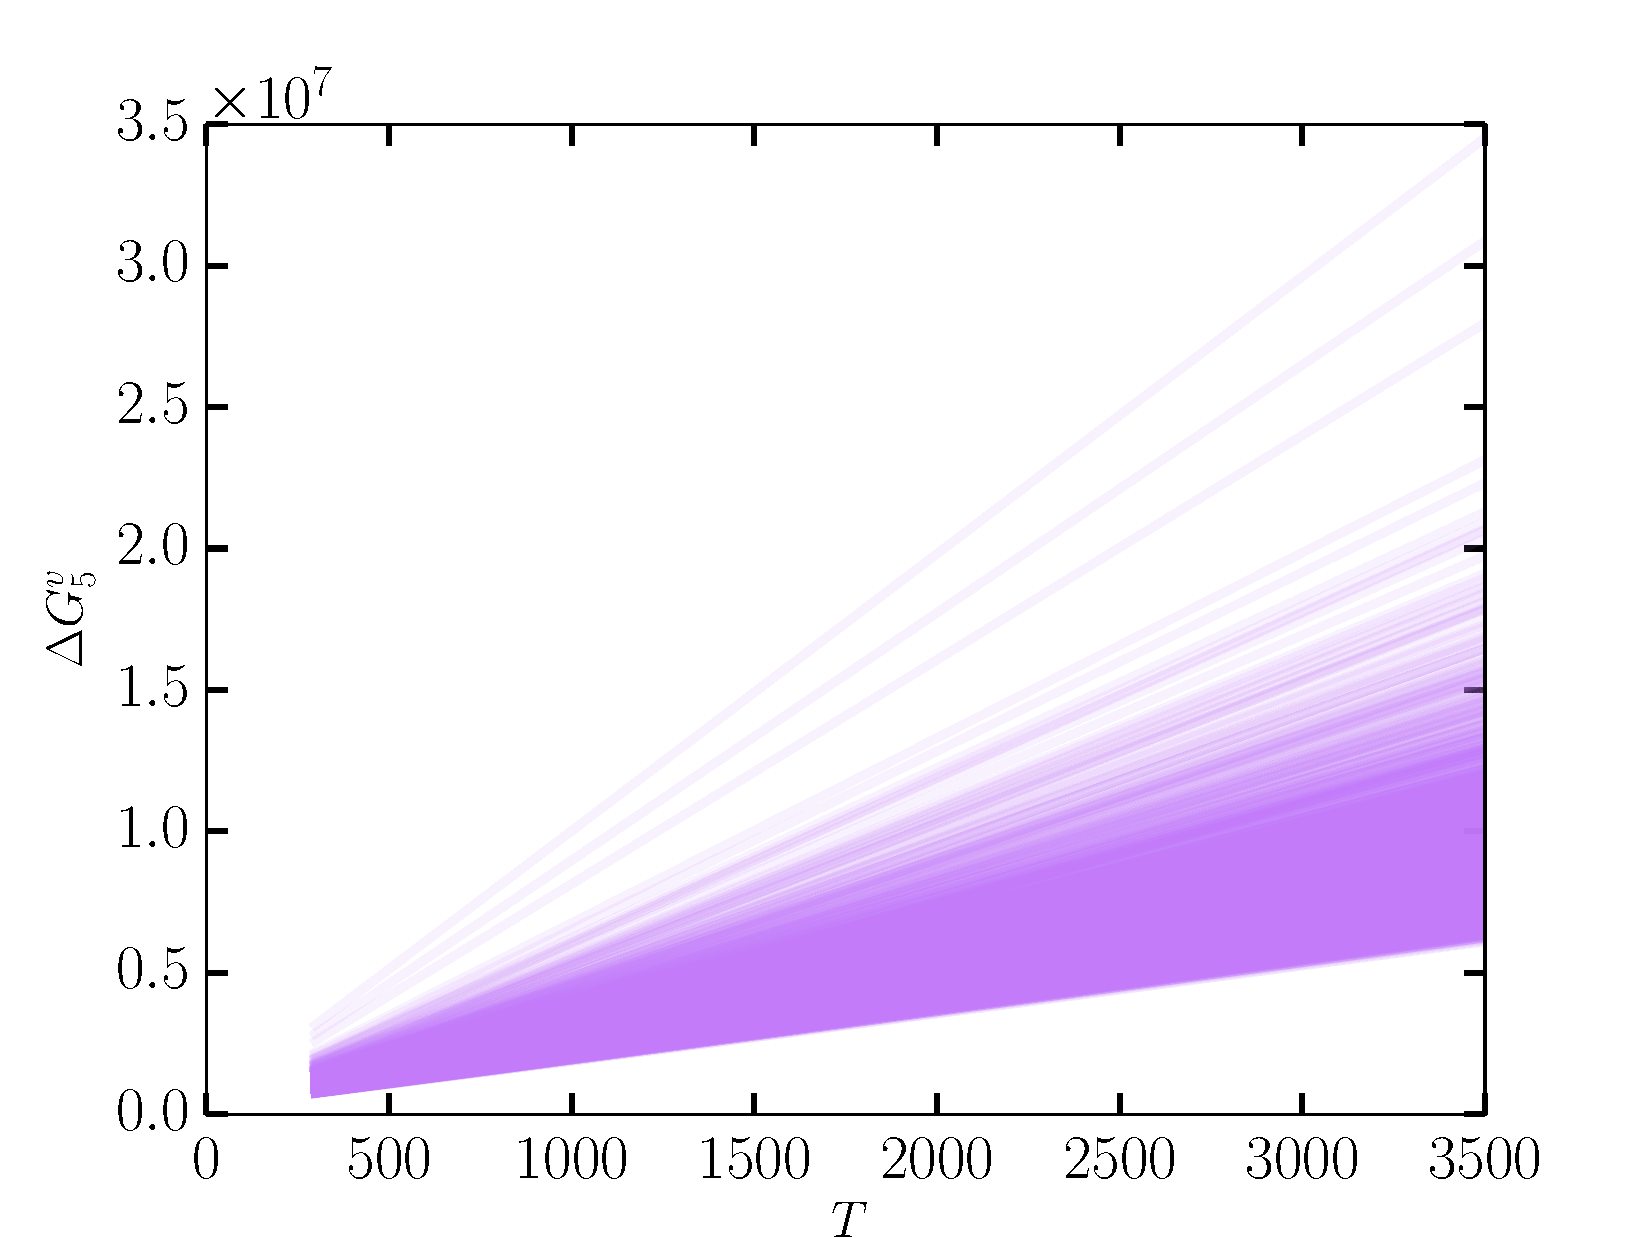
\includegraphics[width=0.7\textwidth]{G5_v.pdf}
    \caption{The Gibbs free energy for virtual reaction $5$
             ($\Delta G_{5}^{\lr{v}}$) from $10000$ realizations 
             of the virtual thermochemistry parameters.  As 
             designed, it remains positive over the entire 
             temperature range.}
    \label{fig:G5v}
  \end{figure}
  
  In the new inadequacy model just outlined, the modified Arrhenius 
  parameters and thermochemistry parameters must be inferred.  As mentioned 
  in the preceding paragraphs, the inference is accomplished with a 
  hierarchical Bayesian method.  The priors for each parameter are given by 
  \begin{align}
    &A_{j} \sim \log\mathcal{N}\lr{\mu_{Aj}, \eta_{Aj}}, \qquad 
    \mu_{Aj} \sim \mathcal{N}\lr{\mu_{Aj}^{\lr{\mu}}, \eta_{Aj}^{\lr{\eta}}}, \qquad 
    \eta_{Aj} \sim \mathcal{J}, \qquad j = 1,\dots, M_{v} \\
    &b_{j} \sim \mathcal{N}\lr{\mu_{bj}, \eta_{bj}}, \qquad 
    \mu_{bj} \sim \mathcal{N}\lr{\mu_{bj}^{\lr{\mu}}, \eta_{bj}^{\lr{\eta}}}, \qquad 
    \eta_{bj} \sim \mathcal{J}, \qquad j = 1,\dots, M_{v} \\
    &E_{j} \sim \mathcal{N}\lr{\mu_{Ej}, \eta_{Ej}}, \qquad 
    \mu_{Ej} \sim \mathcal{N}\lr{\mu_{Ej}^{\lr{\mu}}, \eta_{Ej}^{\lr{\eta}}}, \qquad 
    \eta_{Ej} \sim \mathcal{J}, \qquad j = 1,\dots, M_{v} \\
    &\alpha_{k0} \sim \mathcal{N}\lr{\mu_{\alpha_{k0}}, \eta_{\alpha_{k0}}}, \qquad 
    \mu_{\alpha_{k0}} \sim \mathcal{N}\lr{\mu_{\alpha_{k0}}^{\lr{\mu}}, \eta_{\alpha_{k0}}^{\lr{\eta}}}, \qquad 
    \eta_{\alpha_{k0}} \sim \mathcal{J}, \qquad k = 1,\dots, N_{v} \\
    &\alpha_{ki} \sim \log\mathcal{N}\lr{\mu_{\alpha_{ki}}, \eta_{\alpha_{ki}}}, \qquad 
    \mu_{\alpha_{ki}} \sim \mathcal{N}\lr{\mu_{\alpha_{ki}}^{\lr{\mu}}, \eta_{\alpha_{ki}}^{\lr{\eta}}}, \qquad 
    \eta_{\alpha_{ki}} \sim \mathcal{J}, \quad i > 0, \quad k = 1,\dots, N_{v} \\
    &\gamma_{k} \sim \log\mathcal{N}\lr{\mu_{\gamma k}, \eta_{\gamma k}}, \qquad 
    \mu_{\gamma k} \sim \mathcal{N}\lr{\mu_{\gamma k}^{\lr{\mu}}, \eta_{\gamma k}^{\lr{\eta}}}, \qquad 
    \eta_{\gamma k} \sim \mathcal{J}, \qquad k = 1,\dots, N_{v}
  \end{align}
  where $\mathcal{N}$ is a normal distribution, $\log\mathcal{N}$ 
  represents a log-normal distribution, and $\mathcal{J}$ represents 
  a Jeffrey's prior.  The new model has $69$ dimensions which is about 
  half as many dimensions as the original inadequacy model.

  The majority of this quarter was spent developing the new inadequacy 
  model for chemical kinetics.  The new model has about half as many 
  parameters to infer as the original inadequacy model while providing 
   a more nuanced temperature dependence than the original 
  inadequacy model.  We are now in the process of calibrating the new 
  inadequacy model with data provided by the detailed model.  As in 
  previous quarters, the inadequacy operator will be calibrated using 
  data generated from a detailed model containing $21$ reactions and $8$ 
  species~\cite{yoo2009three}.  Data was generated at three equivalence 
  ratios:  $\phi = 0.5$, $\phi = 1.0$, and $\phi = 2.0$.  Calibration data 
  was taken at $10$ points that captured the essential behavior of the temporal 
  evolution of the temperature.  The reduced model used five reactions and 
  $7$ species~\cite{williams2008detailed}.
  
  Figure~\ref{fig:new_inad_demo} demonstrates that the new inadequacy 
  model is expected to be flexible enough to match the detailed model.  
  The result in Figure~\ref{fig:new_inad_demo} was obtained by 
  hand-tuning the parameters.  In spite of hand-tuning, the result 
  is quite encouraging.
  \begin{figure}[h!]
    \centering
    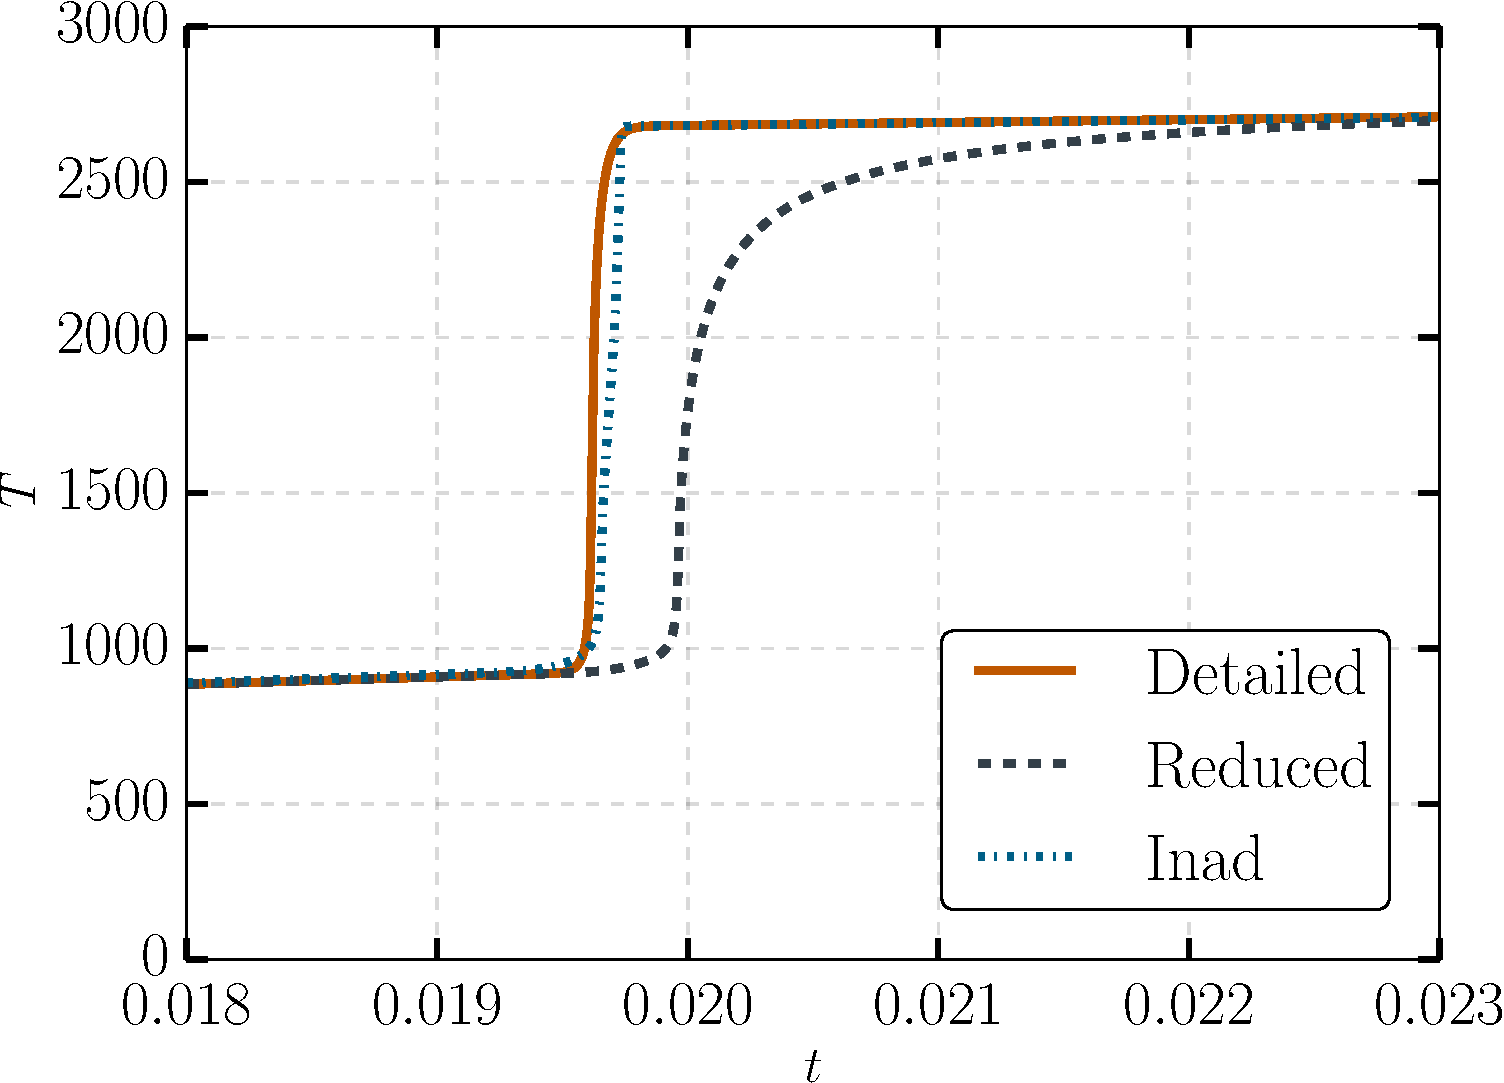
\includegraphics[width=0.7\textwidth]{kinetics_inad_RD.pdf}
    \caption{Time-evolution of the temperature for the detailed, reduced 
             and inadequacy models zoomed to the ignition time.  The 
             hand-tuned inadequacy model matches the truth data very 
             closely indicating that the new inadequacy model may 
             provide the desired flexibility and temperature dependence.}
    \label{fig:new_inad_demo}
  \end{figure}

  \subsection{Discussion}
  Given that hand-tuning the dissociation-recombination 
  inadequacy model gave promising results, we proceeded 
  to start a Bayesian inference.  It quickly became 
  apparent that additional challenges were present.  The 
  inference would sample parameter values such that the 
  numerical integration failed.  Explicit integrators 
  are not expected to perform well on chemical kinetic 
  systems due to the stiffness of chemical kinetics.  We 
  were initially using an explicit integrator (RK45 from GSL) 
  which worked  well for the original inadequacy formulation 
  as well as the detailed and reduced models.  However, 
  the new inadequacy model appeared to be particularly stiff 
  and as a result we switched to an implicit integrator.  
  In principle, an implicit integrator would allow us to 
  take larger time steps and essentially step over the 
  fastest time scales in the system.  One could interpret 
  this feature as being consisten with the quasi-steady state 
  approximation in chemical kinetics.

  We chose to use the CVODE solver provided in the Sundials 
  suite of numerical solvers.  CVODE provides adaptive order 
  BDF methods on top of adaptive time stepping.  The adaptivity 
  is necessary for the solver to actually solve the problem 
  to a specified error tolerance.  In our case, we 
  would prefer to step over the fastest time scales whereas 
  CVODE senses the fastest time scales as part of the 
  adaptive procedure.  This difficulty ultimately caused 
  CVODE to struggle with the inadequacy model to the point 
  where it could often not even find a solution to the problem. 
  We also tried ARKODE which is an IMEX Runge-Kutta solver but 
  had the same issues as CVODE.

  To gain a better understanding of the system, we analyzed 
  the reaction rates from parameter sets that caused the 
  time integration to fail.  The Gibbs free energy constraint 
  gives the greatest difficulties to the time integrator.  To 
  see this, consider the expression for the equilibrium 
  constant~\eqref{eq:ke}.

\bibliographystyle{siam}
\bibliography{chemkin}

\end{document}


